\section{Digitisation}
\label{sec:digi}

The digitisation procedure is aimed at converting Geant4 SimHits into
reconstructed hits, i.e. reproducing what the electronics of the real
detector will do given an analogue signal, with a signal and a noise
component, passed through analogue-to-digital (ADC) convertors, with a
zero-suppression threshold applied to reduce the data volume, and
finally the calibration back to an energy.

Minimum ionising particles (MIPs) will deposit energy according to a
Landau distribution, whose maximum probable value can be used to
convert Geant4 energies into other relevant quantities. 

\subsection{The MIP signal}

The energy deposited by 50 GeV muons per $2.5\times 2.5$ mm$^2$ cells
is shown in figure~\ref{fig:muHits}. On the left the number of cells
with energy deposits are shown as a function of the layer, and on the
right the energy deposits for layers which have one and only one hit.

\begin{figure}[h!]
  \begin{center}
    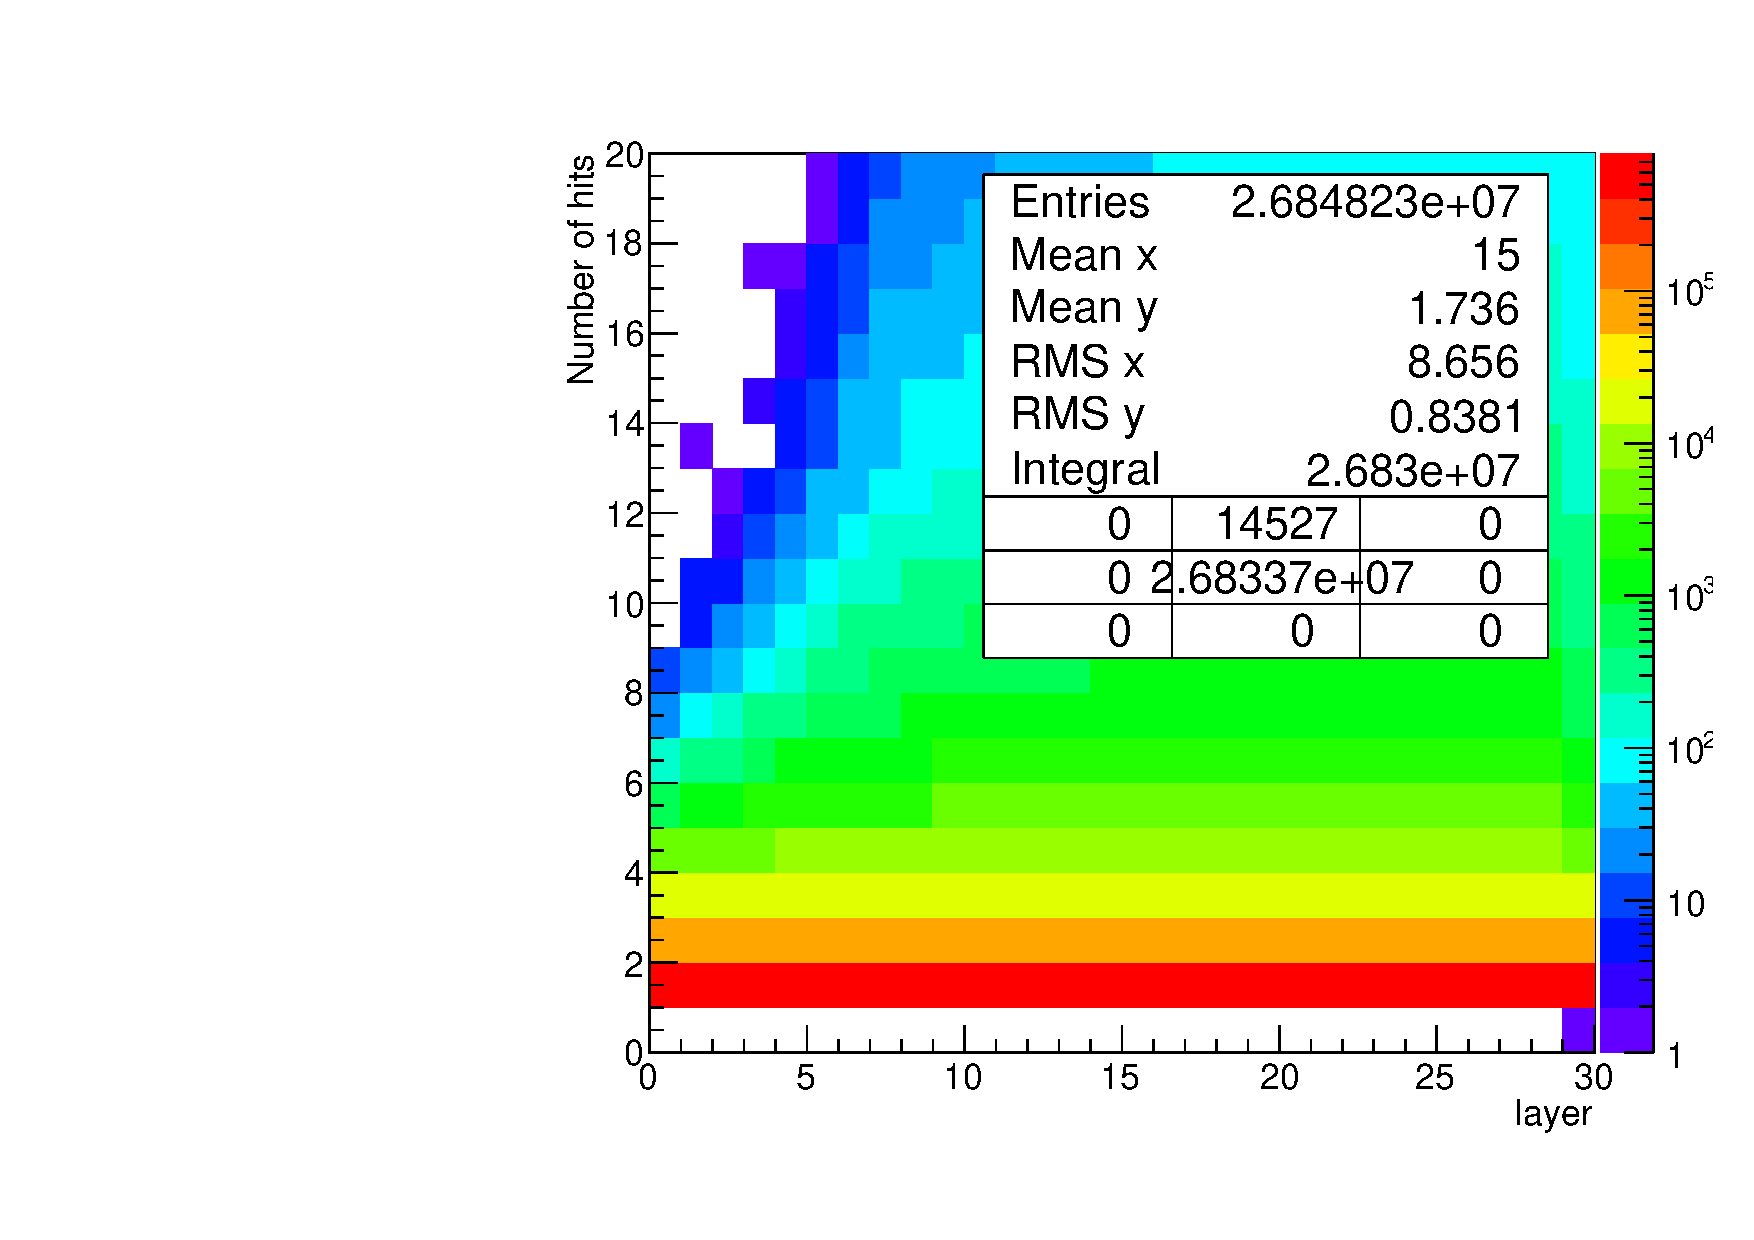
\includegraphics[width=\cmsFigWidth]{figures/mipHits.pdf}
    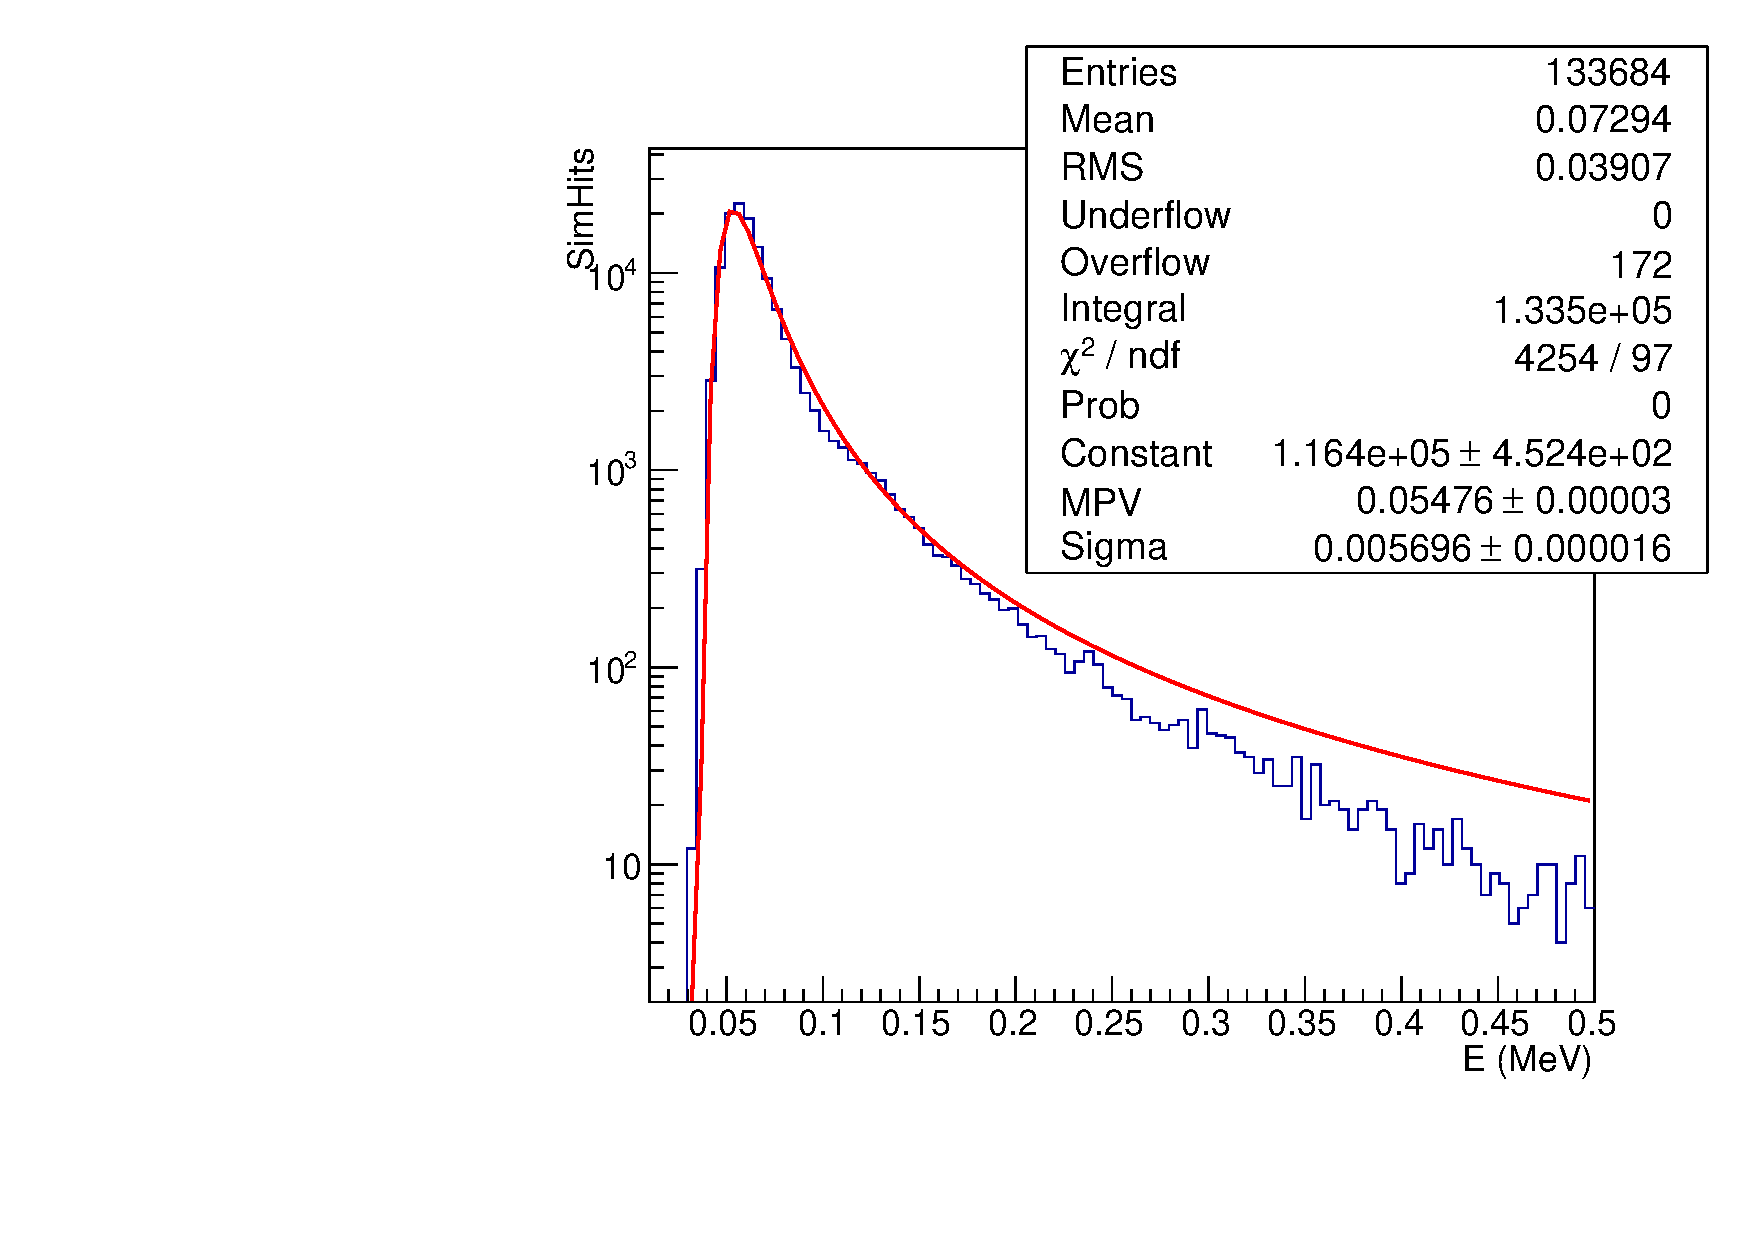
\includegraphics[width=\cmsFigWidth]{figures/mipDepositSel.pdf}
    \caption{}
    \label{fig:muHits}
  \end{center}
\end{figure}

The maximum probable value of the Landau gives the conversion factor
of $$1 \mathrm{MIP} = 0.0545 MeV$$ of energy deposited in Geant4.

\subsection{Electronics calibration and noise}

\subsubsection{MIP to electron conversion}

A MIP will typically create about 75 electron/hole pairs per $\mu$m of
Si. In 200$\mu$m of fully depleted Si, we expect hence about $\simeq
15000$ electrons.

\subsubsection{Dynamic range and MIP to ADC conversion}

The energy deposited by electrons in $1 \times 1$ cm$^2$ Si pads is
shown in figure~\ref{fig:hitE}, on the left for 100 GeV and on the
right for 500 GeV of incoming energy. The dynamic range of the
electronics should hence cover something from below a MIP, in order to
have a calibration peak, and about 1500 MIPs.

\begin{figure}[h!]
  \begin{center}
    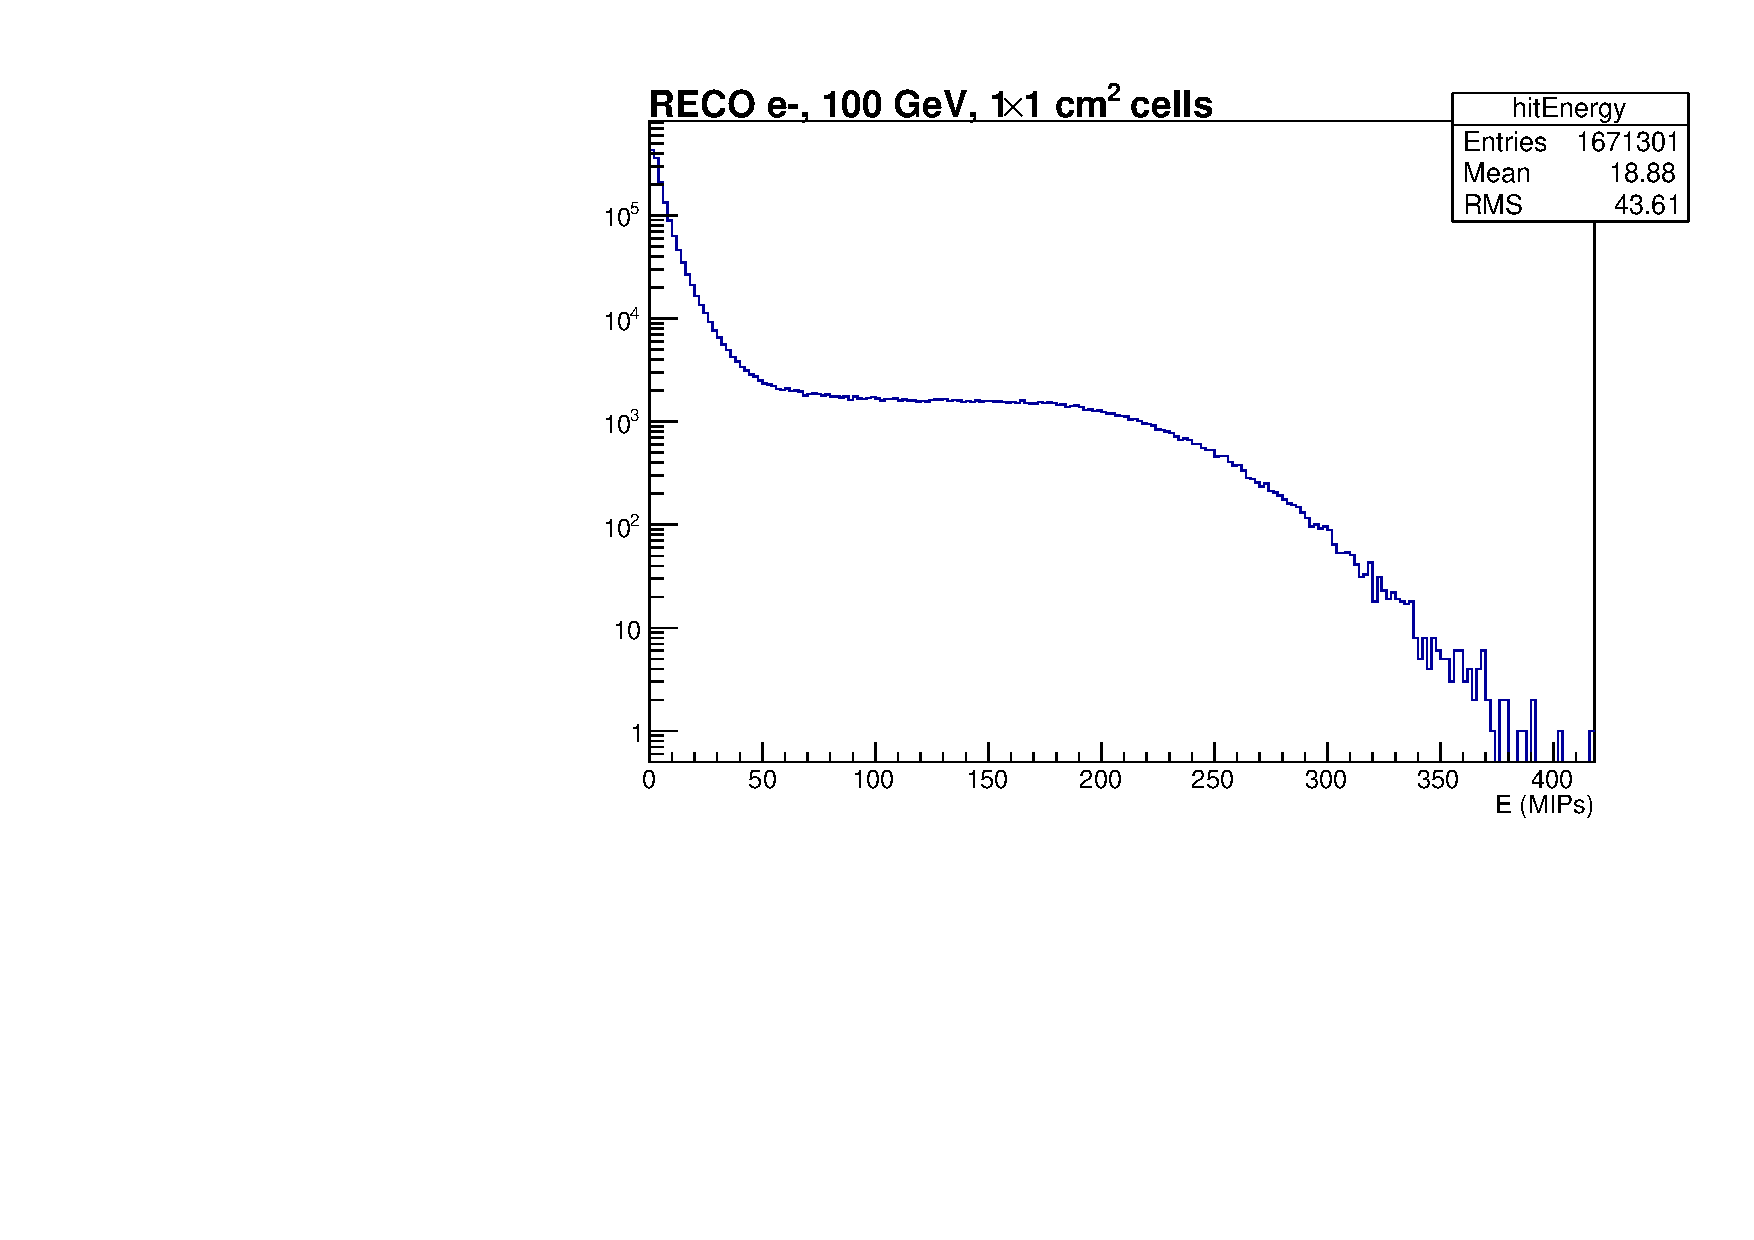
\includegraphics[width=\cmsFigWidth]{figures/HitEnergy_1x1_100GeV.pdf}
    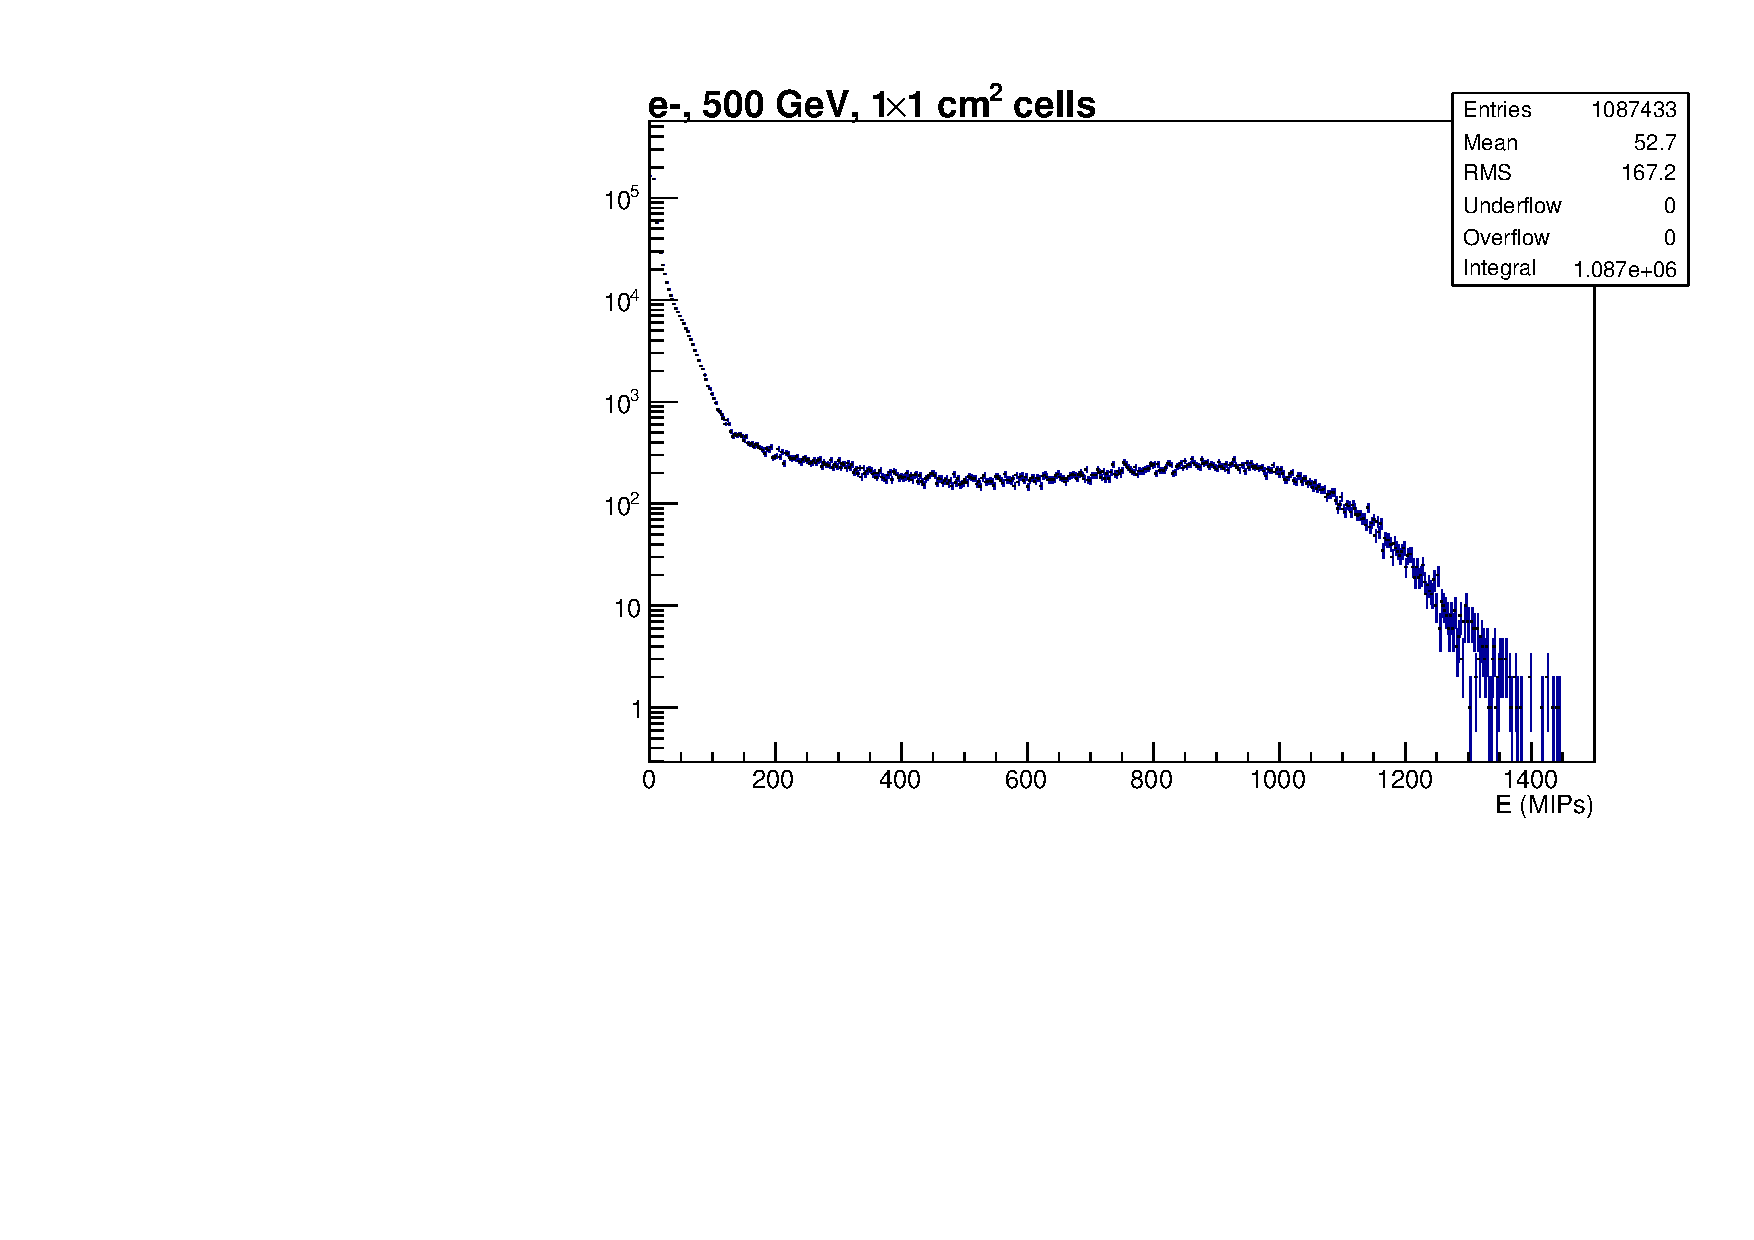
\includegraphics[width=\cmsFigWidth]{figures/HitEnergy_1x1_500GeV.pdf}
    \caption{Energy deposited by electrons per $1 \times 1$ cm$^2$ Si
      pads for 100 GeV (left) and 500 GeV (right) of incoming energy}
    \label{fig:hitE}
  \end{center}
\end{figure}

Three 10-bit ADCs are planned to be used:
\begin{itemize}
\item 10-bit ADC for a range up to 64 MIPs: so 16 ADC counts/MIP or 0.0625 MIP/ADC count.
\item 10-bit ADC for a range up to 1000 MIPs: so 1 ADC counts/MIP.
\item 10-bit ADC for a range up to 10000 MIPs: so 0.1 ADC counts/MIP or 10 MIP/ADC count.
\end{itemize}

The accuracy of the rounding scales as $\frac{x\mathrm{MIPs/ADC
    counts}}{\sqrt{12}}$, so 0.3 MIP for the 1 MIP/ADC count
conversion.

\subsubsection{Noise}

In the CALICE prototype, the signal/noise ratio was measured to be
around 9, so a noise level of about 0.13 MIP. Given this proposal uses
thiner silicon, we can expect a lower signal yield, so comparatively
higher noise. But the noise will decrease with smaller pad sizes, and
with cooling. Note that when using the conversion of 1 MIP / ADC
count, we can expect the noise level to be comparable or lower to the
digitisation accuracy.


\subsubsection{Procedure in software}

The procedure implemented in the standalone simulation is the following:
\begin{itemize}
\item Convert SimHits G4 energy (MeV) to MIPs.
\item Create collection of RecHits with the desired granularity. Baseline: $1 \times 1$ cm$^2$ pads.
\item Add noise in MIPs, included in empty cells.
\item Convert MIPs to ADC counts $\Rightarrow$ DigiHits.
\item Apply threshold: baseline = 5$\times$ noise.
\item Convert ADC counts back to MIPs $\Rightarrow$ RecHits.
\item All parameters are kept configurable for easy scanning.
\end{itemize}

\subsubsection{Impact on the resolution}

\FIXME{Add calibration and resolution curves after digi}